% !TeX root = ..\rapport_13_2.tex
\section{Code coverage}\label{chap:code_coverage}
\begin{figure}[H]
    \centering
    \caption{Coverage for klasser i applikationslaget}
    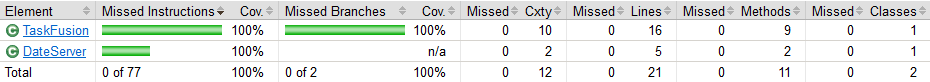
\includegraphics[width = 12cm, keepaspectratio]{ImplementationAndTest/Diagrams/coverage/coverage_app.png}
    \label{fig:coverage_app}
\end{figure}
\begin{figure}[H]
    \centering
    \caption{Coverage for klasser i domænelaget}
    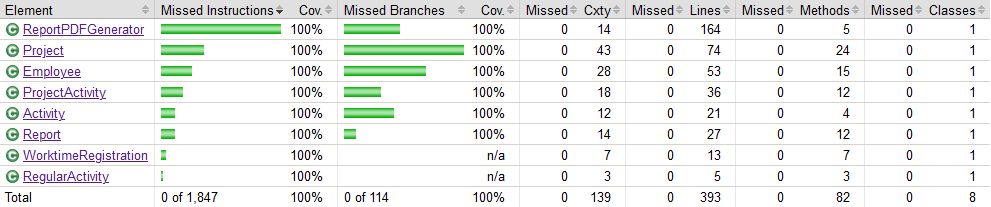
\includegraphics[width = 14cm, keepaspectratio]{ImplementationAndTest/Diagrams/coverage/coverage_domain.png}
    \label{fig:coverage_domain}
\end{figure}
\begin{figure}[H]
    \centering
    \caption{Coverage for exceptions}
    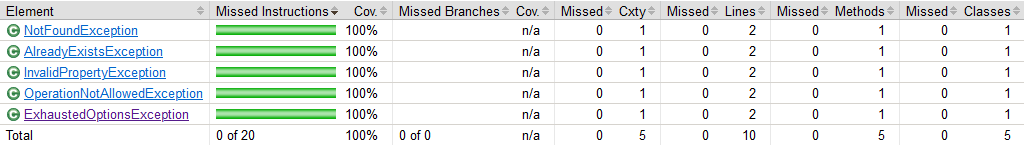
\includegraphics[width = 12cm, keepaspectratio]{ImplementationAndTest/Diagrams/coverage/coverage_exceptions.png}
    \label{fig:coverage_exceptions}
\end{figure}
\begin{figure}[H]
    \centering
    \caption{Coverage for facader}
    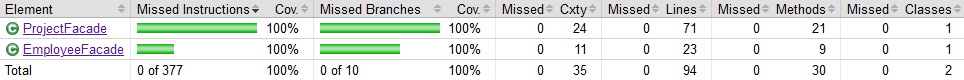
\includegraphics[width = 12cm, keepaspectratio]{ImplementationAndTest/Diagrams/coverage/coverage_facades.png}
    \label{fig:coverage_facades}
\end{figure}
\begin{figure}[H]
    \centering
    \caption{Coverage for hjælperklasser}
    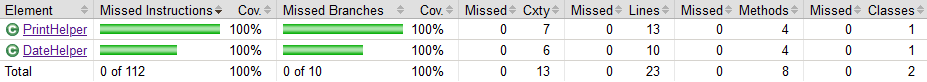
\includegraphics[width = 12cm, keepaspectratio]{ImplementationAndTest/Diagrams/coverage/coverage_helpers.png}
    \label{fig:coverage_helpers}
\end{figure}
\begin{figure}[H]
    \centering
    \caption{Coverage for klasser i persistency-laget}
    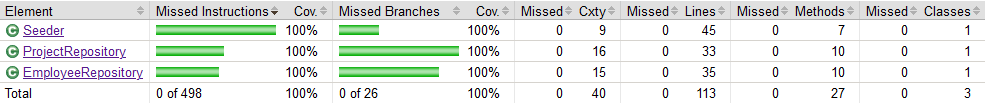
\includegraphics[width = 12cm, keepaspectratio]{ImplementationAndTest/Diagrams/coverage/coverage_persistency.png}
    \label{fig:coverage_persistency}
\end{figure}
\begin{figure}[H]
    \centering
    \caption{Coverage for viewModels}
    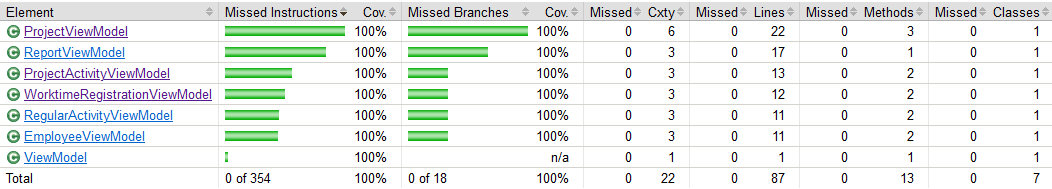
\includegraphics[width = 12cm, keepaspectratio]{ImplementationAndTest/Diagrams/coverage/coverage_viewModels.png}
    \label{fig:coverage_viewModels}
\end{figure}
Som det fremgår af alle ovenstående figurer, er vores coverage på 100 procent, som det forventes ved god praksis af TDD. Målet var først en kende lavere (omtrent 91 procent), hovedsageligt på grund af komplekse if-udtryk, hvor en eller flere delbranches ikke var dækket af de cucumber-features, vi havde skrevet. Med delbranches fra en branch hvor der opstår flere branches pga. permutationer af et if-udtryk med flere conditions. F.eks. giver if (jegErSulten() \&\& jegHarSpist()) fire mulige delbranches: sand (begge er sande), falsk (den første er sand, anden ikke), falsk (omvendt af tidligere), og falsk (ingen af dem er sande). Af den mængde var vi interesserede i færre tilfælde end dem alle, hvorfor coverage faldt fra 100 procent. Dette løstes i nogle tilfælde ved refactoring (ved særligt grelle if-udtryk) eller tilføjelse af nye scenarier, hvis man havde overset et relevant scenarie. De fleste løstes ved tilføjelser til cucumber-scenarier.\\[4mm] En sidste nævneværdig årsag er future-proofing, særligt i generateProjectNumber, hvor lastNum sattes til num, hvis num var større end lastNum. Dette var gjort i starten af projektet med henblik på at gøre koden mindre afhængig af den samling, der eventuelt skulle indeholde alle projekter. I sidste ende lagredes projekter i et Map, der tilfældigvis hasher projektnumrene, så de eksisterer i mappets keySet i stigende rækkefølge indenfor samme år, hvorfor tjekket til sidst fjernedes. 

Hele præsentations-laget er ikke udviklet test-drevent, derfor er hele \textit{cli} mappen ikke inkluderet i code-coverage rapporten. Ved at eskludere hele laget fra code-covarage, har vi også bedre haft styr på validiteten af program-laget, og netop kunne opnå 100\% dækning.